\chapter{Wireless protocols}
\label{chap:wireless}

bla bla

In this chapter, I will describe the Industrial, Scientific and Medical (ISM) 2,4 \(GHz\) radio band in \autoref{sec:ism}.
After that, I will demonstrate each wireless protocol starting with Bluetooth Low Energy in \autoref{sec:ble},
Zigbee in \autoref{sec:zig}, and finally Thread/OpenThread in \autoref{sec:ot}.
\autoref{sec:15_4} will provide an overview of the IEEE 802.15.4 radio specification, of which both Zigbee and Thread is based on.

\section{ISM radio band}
\label{sec:ism}

\section{Bluetooth Low Energy}
\label{sec:ble}

Bluetooth is a low-power, short-range wireless technology developed initially for replacing cables when
connecting devices like mobile phones, headsets, and computers.
It has since evolved into a wireless standard for connecting electronic devices to
form Personal Area Networks (PANs) and ad hoc networks. \cite{Dideles03}

Bluetooth is one of the most popular commodity radios for wireless devices.
As a representative of the frequency hopping spread spectrum radios,
it is a natural alternative to broadcast radios in the context of sensor networks. \cite{Leopold03}

The Bluetooth Special Interest Group (SIG) oversees
the Bluetooth standard and has a membership of over 38,000 companies as of 2023. \cite{bt_history}
The initial specification was made available in 1999.
Since then, the SIG released five core specifications, 5.4 being the latest adoption in 2023. \cite{bt_spec_history}

This thesis will focus mainly on Bluetooth Low Energy due to
its similarity in functionality and utilization to Zigbee and Thread/OpenThread.

blab bla.\cite{ble_primer23}.

\subsection{Introcution}
\label{ble:int}
The Bluetooth 4.0 Core Specification introduced Bluetooth Low Energy (BLE).
It is tempting to represent itself as a smaller and highly optimized version of
its bigger brother, classic Bluetooth. In reality, BLE has an entirely different lineage and design goals.
Initially known as Wibree and created by Nokia, the Bluetooth SIG ultimately embraced the technology.
The focus was to develop a radio standard with the lowest possible power consumption,
specifically optimized for low cost, low bandwidth, low power, and low complexity. \cite{Townsend14}

\subsection{Architecture}
\label{ble:ow}

According to Townsend et al., the Bluetooth Low Energy device can be categorized into
three primary blocks: controller, host, and application.
Each block has one or more layers, as shown in \autoref{fig:ble_arch}.

\begin{figure}[!ht]
    \centering
    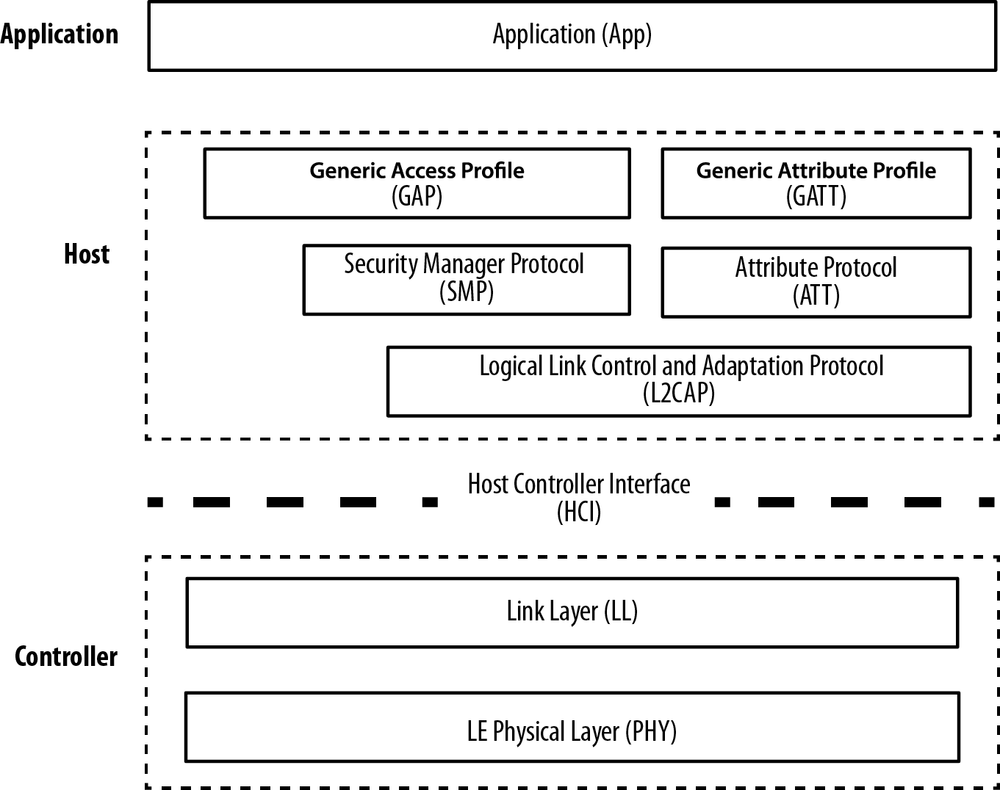
\includegraphics[width=150mm, keepaspectratio]{figures/ble_arch_from_townsend.png}
    \caption{The BLE protocol stack. (Source: Figure 2-1 \cite{Townsend14})}
    \label{fig:ble_arch}
\end{figure}

The layers defined in \autoref{fig:ble_arch} provide the required functionality to operate.

\subsection{Physical layer}
\label{ble:phy}

The physical layer (PHY) contains all necessary analog communication circuitry.
The radio uses the 2.4 GHz ISM band to communicate.
This band is divided into 40 channels or subbands from 2.400 GHz to 2.4835 GHz,
each subband using 2 MHz of bandwidth. (Yin et al., 2019)
This division can be seen in \autoref{fig:ble_phy}.
There are three dedicated advertising subbands for connection setup and
broadcast messages; the remaining 37 are known as general-purpose channels.

\begin{figure}[!ht]
    \centering
    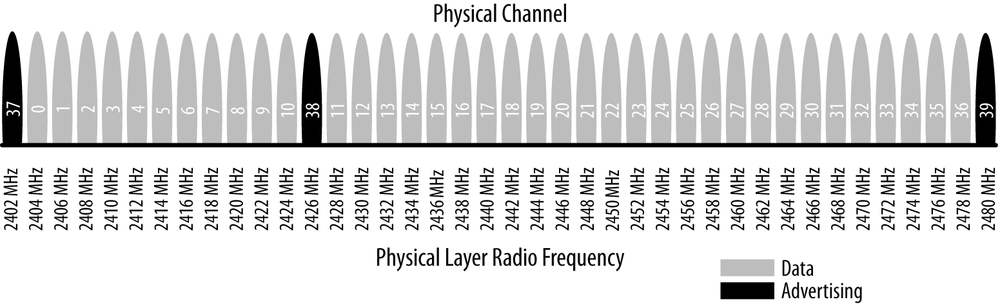
\includegraphics[width=150mm, keepaspectratio]{figures/ble_phy.png}
    \caption{Channel allocation. (Source: Figure 2-2 \cite{Townsend14})}
    \label{fig:ble_phy}
\end{figure}

J. Yin et al. \cite{Yin:19} showed that from Core Specification 5, a novel
modulation scheme was introduced in the standard.
This feature allowed radio modules to use up all 2 MHz of bandwidth,
thus significantly increasing the maximum throughput.

\subsection{Link layer}
\label{ble:link}
The Core Specification's volume six (Low Energy Controller volume),
part B defines the Bluetooth Low Energy Link Layer's specification.

The Link Layer is the component that directly communicates with the PHY.
It is typically a blend of custom hardware and software. \cite{Townsend14}


\subsection{Generic Access Profile}
\label{ble:gap}

\subsection{Generic Attibute Profile}
\label{ble:gatt}

\section{IEEE 802.15.4}
\label{sec:15_4}

bla bla

\section{Zigbee}
\label{sec:zig}

Zigbee is a wireless communication protocol specifically designed for
applications requiring low-power consumption and short-range communication.
It operates on the IEEE 802.15.4 standard and provides a reliable and efficient way
for devices to connect and communicate with each other.
Zigbee is a frequently used technology in home automation, industrial control systems,
and various other applications related to the Internet of Things (IoT).
It supports mesh networking, allowing devices to relay data to extend the network
coverage. Zigbee is known for its low power consumption, simple implementation, and
ability to support a large number of devices in a network.

\url{https://www.academia.edu/73196763/A_Survey_of_ZigBee_Wireless_Sensor_Network_Technology_Topology_Applications_and_Challenges}

\url{https://issuu.com/ijtsrd.com/docs/399_literature_survey_on_zigbee_iee}
\url{https://www.sciencedirect.com/topics/engineering/zigbee-protocol}

\section{Thread/OpenThread}
\label{sec:ot}
openthread.

\url{https://ieeexplore.ieee.org/abstract/document/8767079}
\url{https://ieeexplore.ieee.org/abstract/document/8373620}
\url{https://ieeexplore.ieee.org/abstract/document/10022228}
\url{https://ieeexplore.ieee.org/abstract/document/9058170}
\url{https://dl.acm.org/doi/abs/10.1145/3507657.3528544}
\url{https://www.diva-portal.org/smash/record.jsf?pid=diva2%3A1040491&dswid=1593}
\url{https://upcommons.upc.edu/handle/2117/101928}
\url{https://ieeexplore.ieee.org/abstract/document/8106811}
\url{https://ieeexplore.ieee.org/abstract/document/8592759}
\url{https://ieeexplore.ieee.org/abstract/document/8374875}
\url{https://www.diva-portal.org/smash/record.jsf?pid=diva2%3A1282697&dswid=-3708}
\url{https://ieeexplore.ieee.org/abstract/document/8586865}
\url{https://link.springer.com/chapter/10.1007/978-3-030-70080-5_9#Sec8}